\chapter{Foundations}
\label{cha:foundations}

\section{Use Case Motivation}

The company BestRental wants to develop a monitoring solution for its BestRentalPoC system
to collect metrics that are meant to assist the company in operating the BestRentalPoC.
The system will be operated by QA Engineers, system operators, and a project manager.
Before developing the monitoring solution, the team tasked with developing the solution,
interview the different roles to find out how they will use the solution
and what their tasks and responsibilities are.
QA Engineers are responsible for the reliability of BestRentalPoC.
To ensure the reliability of the system, they want to know when requests to the system fail and
trigger errors, so that they can fix them.
For them to better understand errors, they want to know how often errors occur and from which services,
inside of BestRentalPoC, they originate.
The system operators run the BestRentalPoC. They need to make sure that at any point in time
BestRentalPoC has enough instances of all of its services available to serve all incoming requests.
Because BestRental wants to operate profitably, they can't just create as many instances as they like,
and they need to shut down instances when they are not needed.
To assist them with their task, they want to know how high the resource usage of each instance is
and how many requests are coming into the system. The resources that they want to track for each
instance are the instance's CPU and memory usage.
The project manager's yearly bonus is tied to how profitable the BestRentalPoC operates.
To ensure that he gets his bonus, the project manager wants to track the operating costs of the complete system.
Additionally, he needs to how high the operating costs of each service are, so that he can
allocate development time to increase the efficiency of a service, making it more profitable.
After the interviews, the development notes that all types of users of the monitoring solution
want to be able to do five different things.
Firstly, they want to be able to create a dashboard for a metric that displays its current and historic values.
When viewing a dashboard they also want to be able to run queries on the metric to, for example, get
its value at a specific point in time.
Because the users can't constantly watch all of their dashboards, they want to be able to create
alerts for a metric that will be triggered when the metric exceeds a set value.
When a metric exceeds a value set for an alert, the users want to receive the alert so that they can act on it.
The developers also know that the solution needs to be able to do three main things to accomplish
the requested features.
Firstly, the solution needs to collect metrics from BestRentalPoC,
it then needs to analyze the collected data, and lastly, it needs to conditionally send out alerts
for metrics.

\section{Use Case Descriptions}

% \begin{figure}[h]
% 	\centering
% 	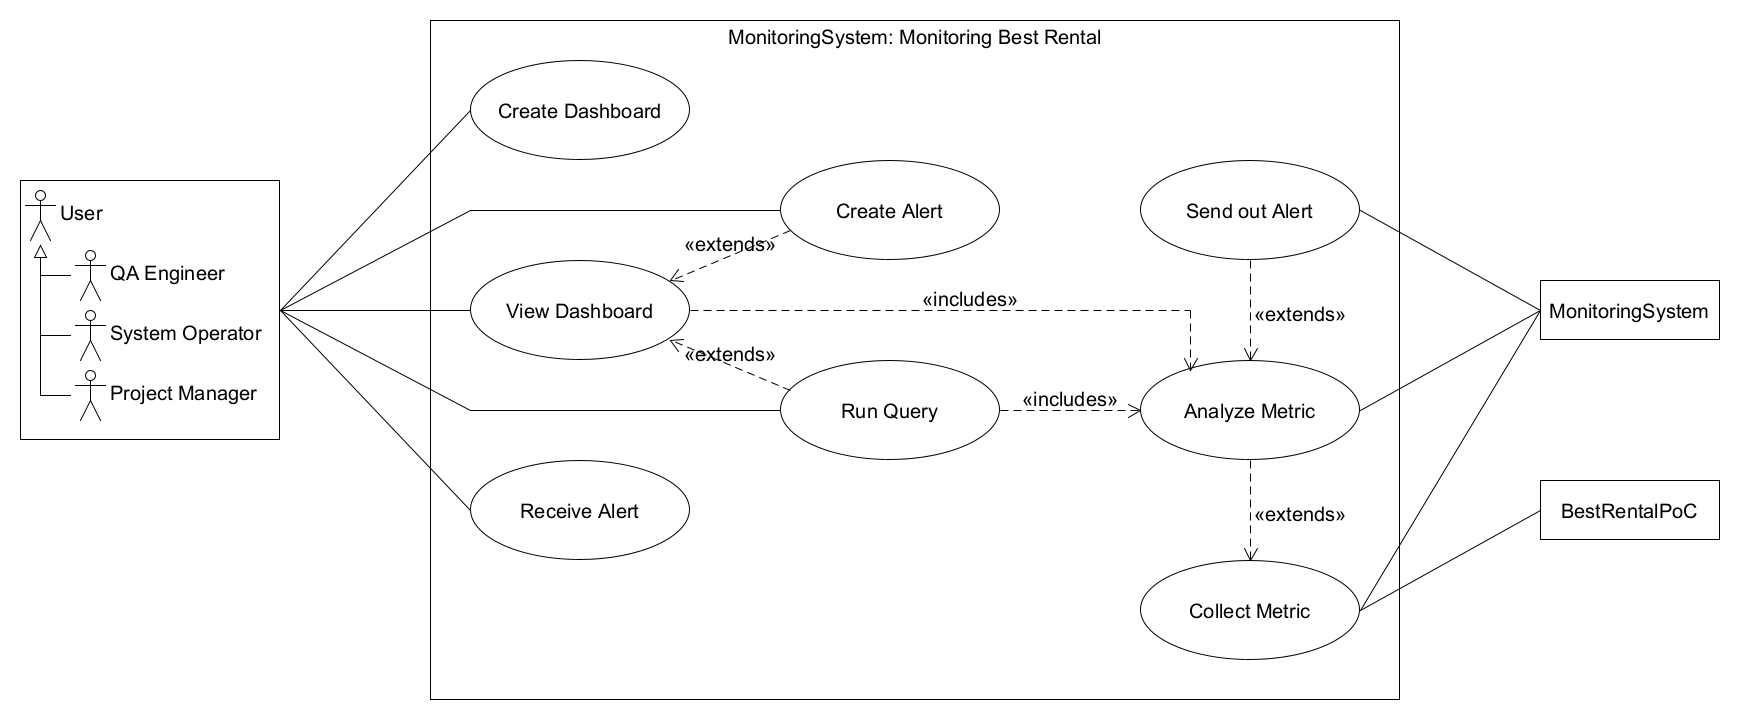
\includegraphics[width=\textwidth]{figures/use_case_monitoring_bestrental.png}
% 	\caption{Use Case: Monitoring BestRental}
% 	\label{fig:use_case_monitoring_best_rental}
% \end{figure}

\vspace{0.5cm}
\begin{lstlisting}[caption = {Use Case Description: Monitoring BestRental}, label = {lis:use_case_description_monitoring_bestrental}, style = kit-cm, language=] 
Title: A Developer creates metrics and dashboards for BestRentalPoC

Primary Actors: Developer
Secondary Actors: MonitoringSystem

Preconditions:
- The Developer has a valid account for the monitoring system
Postconditions:
- The metrics "total accumulated cost", "average CPU usage per service", "average memory usage per service", and "total failed requests" have been created
- Dashboards for the new metrics have been created


Flow:
1. The Developer sets up a new metric "total accumulated cost"
2. The Developer sets up a new metric "average CPU usage per service"
3. The Developer sets up a new metric "average memory usage per service"
4. The Developer sets up a new metric "total failed requests"
5. The Developer logs into the monitoring system
6. The Developer creates a dashboard for the metric "total accumulated cost"
7. The Developer creates a dashboard for the metric "average CPU usage per service"
8. The Developer creates a dashboard for the metric "average memory usage per service"
9. The Developer creates a dashboard for the metric "total failed requests"
10. The Developer logs out of the monitoring system

\end{lstlisting}

\vspace{0.5cm}
\begin{lstlisting}[caption = {Use Case Description: A project manager monitors the cost of BestRentalPoC}, label = {lis:use_case_description_project_manager}, style = kit-cm, language=] 
Title: A project manager monitors the cost of BestRentalPoC

Primary Actors: Project Manager
Secondary Actors: MonitoringSystem

Preconditions:
- The Project Manager has a valid account for the monitoring system
- The metric "total accumulated cost" has been set up
- A dashboard for the metric "total accumulated cost" exists
Postconditions:
- The Project Manager received an alert for the metric "total accumulated cost" via email

Flow:
1. The Project Manager logs into the monitoring system
2. The Project Manager views the dashboard for the metric "total accumulated cost"
3. The Project Manager creates an alert for the metric "total accumulated cost" when the value exceeds 10,000
4. The Project Manager runs a query on the metric "total accumulated cost" to see its value one month ago
5. The Project Manager logs out of the monitoring system
6. The MonitoringSystem detects that the value of the metric "total accumulated cost" exceeds 10,000
7. The MonitoringSystem sends the Project Manager an alert via email
8. The Project Manager receives an alert for the metric "total accumulated cost" via email

Alternative flows:
7a. The value of the metric "total accumulated cost" does not exceed 10,000
	7a1. The MonitoringSystem does not send out an alert for the metric "total accumulated cost" via email
8a. The value of the metric "total accumulated cost" does not exceed 10,000
	8a1. The Project Manager does not receive an alert for the metric "total accumulated cost" via email

Information requirements:
- Values for the metric "total accumulated cost" reaching back at least one month
\end{lstlisting}

\vspace{0.5cm}
\begin{lstlisting}[caption = {Use Case Description: A system operator monitors the cost of BestRentalPoC}, label = {lis:use_case_description_system_operator}, style = kit-cm, language=] 
Title: A system operator monitors the cost of BestRentalPoC

Primary Actors: System Operator
Secondary Actors: MonitoringSystem

Preconditions:
- The System Operator has a valid account for the monitoring system
- The metric "average CPU usage per service" has been set up
- The metric "average memory usage per service" has been set up
- A dashboard for the metric "average CPU usage per service" exists
- A dashboard for the metric "average memory usage per service" exists
Postconditions:
- The System Operator received an alert for the metric "average CPU usage per service" via email
- The System Operator received an alert for the metric "average memory usage per service" via email

Flow:
1. The System Operator logs into the monitoring system
2. The System Operator views the dashboard for the metric "average CPU usage per service"
3. The System Operator creates an alert for the metric "average CPU usage per service" when the value exceeds 95%
4. The System Operator runs a query on the metric "average CPU usage per service" to see its value one month ago
5. The System Operator views the dashboard for the metric "average memory usage per service"
6. The System Operator creates an alert for the metric "average memory usage per service" when the value falls below 10%
7. The System Operator runs a query on the metric "average memory usage per service" to see its value one month ago
8. The System Operator logs out of the monitoring system
9. The MonitoringSystem detects that the value of the metric "average CPU usage per service" exceeds 95%
10. The MonitoringSystem sends the Project Manager an alert for the metric "average CPU usage per service" via email
11. The Project Manager receives an alert for the metric "average CPU usage per service" via email
12. The MonitoringSystem detects that the value of the metric "average memory usage per service" is below 10%
13. The MonitoringSystem sends the Project Manager an alert for the metric "average memory usage per service" via email
14. The Project Manager receives an alert for the metric "average memory usage per service" via email

Alternative flows:
10a. The value of the metric "average CPU usage per service" does not exceed 95%
	10a1. The MonitoringSystem does not send out an alert for the metric "average CPU usage per service" via email
11a. The value of the metric "average CPU usage per service" does not exceed 95%
	11a1. The System Operator does not receive an alert for the metric "average CPU usage per service" via email
13a. The value of the metric "average memory usage per service" is not below 10%
	13a1. The MonitoringSystem does not send out an alert for the metric "average memory usage per service" via email
14a. The value of the metric "average memory usage per service" is not below 10%
	14a1. The System Operator does not receive an alert for the metric "average memory usage per service" via email

Information requirements:
- Values for the metric "average CPU usage per service" reaching back at least one month
- Values for the metric "average memory usage per service" reaching back at least one month
\end{lstlisting}

\vspace{0.5cm}
\begin{lstlisting}[caption = {Use Case Description: A QA engineer monitors the cost of BestRentalPoC}, label = {lis:use_case_description_qa_engineer}, style = kit-cm, language=] 
Title: A QA engineer monitors the cost of BestRentalPoC

Primary Actors: QA Engineer
Secondary Actors: MonitoringSystem

Preconditions:
- The QA Engineer has a valid account for the monitoring system
- The metric "total failed requests" has been set up
- A dashboard for the metric "total failed requests" exists
Postconditions:
- The System Operator received an alert for the metric "total failed requests" via email

Flow:
1. The QA Engineer logs into the monitoring system
2. The QA Engineer views the dashboard for the metric "total failed requests"
3. The QA Engineer creates an alert for the metric "total failed requests" when the value exceeds 100
4. The QA Engineer runs a query on the metric "total failed requests" to see its value one month ago
5. The QA Engineer logs out of the monitoring system
6. The MonitoringSystem detects that the value of the metric "total failed requests" exceeds 100
7. The MonitoringSystem sends the System Operator an alert via email
8. The System Operator receives an alert for the metric "total failed requests" via email

Alternative flows:
7a. The value of the metric "total failed requests" does not exceed 100
	7a1. The MonitoringSystem does not send out an alert for the metric "total failed requests"
8a. The value of the metric "total failed requests" does not exceed 100
	7a1. The System Operator does not receive an alert for the metric "total failed requests" via email

Information requirements:
- Values for the metric "total failed requests" reaching back at least one month
\end{lstlisting}


\vspace{0.5cm}
\begin{lstlisting}[caption = {Use Case Description: The MonitoringSystem collects metrics from BestRentalPoC}, label = {lis:use_case_description_monitoring_system}, style = kit-cm, language=] 
Title: The MonitoringSystem collects metrics from BestRentalPoC

Primary Actors: MonitoringSystem
Secondary Actors: BestRentalPoC

Preconditions:
- The MonitoringSystem is configured to collect the metric "total accumulated cost"
- The MonitoringSystem is configured to collect the metric "average CPU usage per service"
- The MonitoringSystem is configured to collect the metric "average memory usage per service"
- The MonitoringSystem is configured to collect the metric "total failed requests"
Postconditions:
- The MonitoringSystem has the latest value for the metric "total accumulated cost" stored
- The MonitoringSystem has the latest values for the metric "average CPU usage per service" stored
- The MonitoringSystem has the latest values for the metric "average memory usage per service" stored
- The MonitoringSystem has the latest value for the metric "total failed requests" stored

Flow:
1. The MonitoringSystem requests the latest value for the metric "total accumulated cost" from each service
2. Each service from BestRentalPoC sends its latest value for the metric "total accumulated cost" to the MonitoringSystem
3. The MonitoringSystem combines the values for the metric "total accumulated cost" from each service into one value
4. The MonitoringSystem stores the latest value for the metric "total accumulated cost"
5. The MonitoringSystem requests the latest value for the metric "average CPU usage per service" from each service
6. Each service from BestRentalPoC sends its latest value for the metric "average CPU usage per service" to the MonitoringSystem
7. The MonitoringSystem stores the latest values for the metric "average CPU usage per service"
8. The MonitoringSystem requests the latest value for the metric "average memory usage per service" from each service
9. Each service from BestRentalPoC sends its latest value for the metric "average memory usage per service" to the MonitoringSystem
10. The MonitoringSystem stores the latest values for the metric "average memory usage per service"
11. The MonitoringSystem requests the latest value for the metric "total failed requests" from each service
12. Each service from BestRentalPoC sends its latest value for the metric "total failed requests" to the MonitoringSystem
13. The MonitoringSystem combines the values for the metric "total failed requests" from each service into one value
14. The MonitoringSystem stores the latest value for the metric "total failed requests"
	
Information Requirements: 
- New values for the metric "total accumulated cost"
- New values for the metric "average CPU usage per service"
- New values for the metric "average memory usage per service"
- New values for the metric "total failed requests"
\end{lstlisting}